%\documentclass[]{article}
\documentclass[smallextended]{svjour3}    


%------------------------------------------------------------------------------% onecolumn (second format)
\usepackage{graphicx}
% \usepackage{subcaption} 
\usepackage[caption=false]{subfig}
\usepackage{multirow}
\usepackage{booktabs}
\usepackage{hyperref}
\usepackage{array}
\usepackage{capt-of}

\RequirePackage{etex} 
%questions and answers
\usepackage{enumitem}
\newenvironment{questions}{\begin{enumerate}[label=\bfseries\alph*.]\bfseries}
	{\end{enumerate}}
\newenvironment{answer}{\par\normalfont}{}
\usepackage[title]{appendix}

% bibliography
\usepackage[backend=biber,
url=false,
doi=false,
eprint=false,
isbn=false,
giveninits,
uniquename=init,
citestyle=authoryear,
maxcitenames=1,
minbibnames = 6,
maxbibnames = 6,
bibstyle=apa]{biblatex}
\addbibresource{scisci_embedding.bib}

\DeclareSourcemap{
	\maps[datatype=bibtex]{
		\map{
			\step[fieldset=issn, null]
			\step[fieldset=url, null]
			\step[fieldset=doi, null]
			\step[fieldset=eprint, null]
		}
	}
}

%\usepackage{natbib}

% comments
\usepackage{xargs} % Use more than one optional parameter in a new commands
\usepackage[pdftex,dvipsnames]{xcolor}  % Coloured text etc.
%\usepackage[colorinlistoftodos,prependcaption,textsize=tiny]{todonotes}
%\newcommandx{\note}[2][1=]{\todo[linecolor=red,backgroundcolor=red!25,bordercolor=red,#1]{#2}}
%\newcommandx{\todo}[2][1=]{\todo[linecolor=blue,backgroundcolor=blue!25,bordercolor=blue,#1]{#2}}
%\newcommandx{\something}[2][1=]{\todo[linecolor=OliveGreen,backgroundcolor=OliveGreen!25,bordercolor=OliveGreen,#1]{#2}}
% comments

% tikz
\usepackage{xcolor}
\usepackage{tikz-network}
\usepackage{tikz}

\usepackage{algorithm}
\usepackage[noend]{algpseudocode}


\usepackage{amsmath}
\usepackage{amssymb} 

\definecolor{frenchblue}{rgb}{0.0, 0.45, 0.73}
\definecolor{etonblue}{rgb}{0.59, 0.78, 0.64}
\definecolor{darkcoral}{rgb}{0.8, 0.36, 0.27}
\definecolor{urobilin}{rgb}{0.88, 0.68, 0.13}
\definecolor{wisteria}{rgb}{0.79, 0.63, 0.86}

% paths

\graphicspath{{plots/}{img/}}


%%%%%%%%%%%%%%%%%%%%%%%%%%%%
%for comments
\newcommand\JP[1]{\textcolor{magenta}{JP: #1}}
%%%%%%%%%%%%%%%%%%%%%%%%%%%


%opening
\title{Snippets left out from the article of Science of Science}
\titlerunning{The Science of Science Embedding Spaces}
\author{Diego Kozlowski}

\institute{}
\date{}

%------------------------------------------------------------------------------
\begin{document}
	\maketitle
	%------------------------------------------------------------------------------
	\section{Results}
	\label{sec:Results}
	%------------------------------------------------------------------------------
	
\subsection{Comparing Differences between the Semantic and Relational Space}
	\label{sec:Differences}
	%------------------------------------------------------------------------------
	After studying the overall quality of the different models, we focus on those that have the best performance in both the semantic and the relational space. For the latter, we select the GCN using BERT embeddings as features. For the semantic space, we mainly focus on the BERT model, but also show some results for the LDA model for comparison. In this section, we show how the embedding representation of articles change in the semantic and relational space. For this, we compare the results on four different topics largely studied in the science of science field: First, the representation of collaboration patterns; second, the Matthew effect; third, we perform a country level analysis; and finally, the quantitative-qualitative divide in the field. The goal is to check if this different phenomenon are encoded in the resulting embedding, and how their representations differs within the different proposed models.
	%------------------------------------------------------------------------------

	
	%------------------------------------------------------------------------------
	\paragraph{\textbf{The Matthew effect}}
	%------------------------------------------------------------------------------

	The Matthew effect \parencite{merton_sociology_1974} states that highly cited articles have a higher chance of being cited again. Figure~\ref{fig:cosine_similarity_gnn} reflects on this via the collaboration patterns, while Figure~\ref{fig:tsnegnnjournal} also shows a correlation of articles by the number of citations. Given that the decoder function of the GNN is the inner product of the embedding (see Section~\ref{sec:Embeddings}), a higher norm in the vector representation of an article will correspond with a higher link probability, i.e. citation relation, with all other articles. To test if the embeddings are able to capture the Matthew effect, we divided the articles by their number of total citations in the Scopus dataset, by the quartiles of the number of citations distribution, and those with zero citations.  Those articles with lower citations than the 25\% threshold correspond to the group \textit{lower}, those between 25\% and 50\% to the \textit{mid-low}, between 50\% and 75\% to \textit{mid-high} and those articles with more than the 75\%  threshold belong to the group \textit{high}. When calculating the average Frobenius norm of articles' embedding at these citation levels in the different models, we confirm that while the GNN generates a higher value for the highly cited articles, the BERT, Doc2Vec and LDA models don't follow this pattern\footnote{In Appendix~\ref{sec:frobenius_norm} we show a complementary figure for this analysis.}. This implies that the GNN is able to encode in the embedding the Matthew effect, but this cannot be seen when the embeddings are exclusively based on text. 
	
	%------------------------------------------------------------------------------
	\paragraph{\textbf{Country-level analysis}}
	%------------------------------------------------------------------------------

	In the same way we built a BERT embedding by averaging the word embeddings of each document, we can build a hierarchical representation of entities by averaging its components. One of the dimensions of analysis is the role of countries in the science of science community. For this, we took the first author's organisational affiliation to ascribe a geographical location to an article. This does not necessarily mean that an article has been written in that country, but it gives us a proxy for the geographical distribution of scientific work and allows us to reconstruct the average position of countries in the embedding. Using the cosine similarity between countries, Figure~\ref{fig:average_embedding} shows the average similarity of a country with respect to all others in the GNN (horizontal axis) and BERT (vertical axis) embeddings. This means that we are comparing the semantical proximity on the vertical axis against the structural network-based proximity on the horizontal axis. Results show that there is a centre of gravity of science production~\parencite{Zhang2015} that includes most of the English-speaking countries, (Western) Europe and (East) Asia. Close to the core, we can also find some countries from (South) America and (East) Europe. South Africa is the only country from its continent close to the centre. Results also show that the BERT cosine similarity is almost always higher than 0.8, while the GNN ranges between $-0.5$ and $0.5$. This means that the semantic representation is in general very similar between all countries, while in the structural representation countries are never too close, and many of them are even in the opposite direction of most of the other countries. The presented results can be interpreted as follows: While researchers in science of science from all countries,within this journals, work on more or less similar content, the relevance that the academic community gives to their work is highly skewed. For example, in the case of Uruguay, the average BERT cosine similarity, i.e., based on the textual content of the articles, from this country and all others, is almost $0.95$, a really high value considering cosine similarity moves between $-1$ and $1$. On the other hand, its citation-based cosine similarity is less than $-0.35$, which means that it is in an opposite direction with respect to most of the countries. As we mentioned in the Section~\ref{sec:Data}, this analysis is limited due to the limits of the dataset. We cannot fully account for scientific production outside the countries that appear here as peripheral. Including journals from other regions and languages would most probably change the layout of the results, specially for the semantic embeddings~\parencite{beigel_introduction_2014}. In this sense, we have to limit the scope of interpretation to the fact that, \textit{within these journals}, the topics discussed do not vary much. Nevertheless, this result is inline with many other studies in the field on the unequal distribution of prestige, at least in the international journals \parencite{demeter_world-systemic_2020, king_power_2011,bonitz_characteristics_1997, merton_sociology_1974}. 
	
	\begin{figure}[!t]
		\centering
		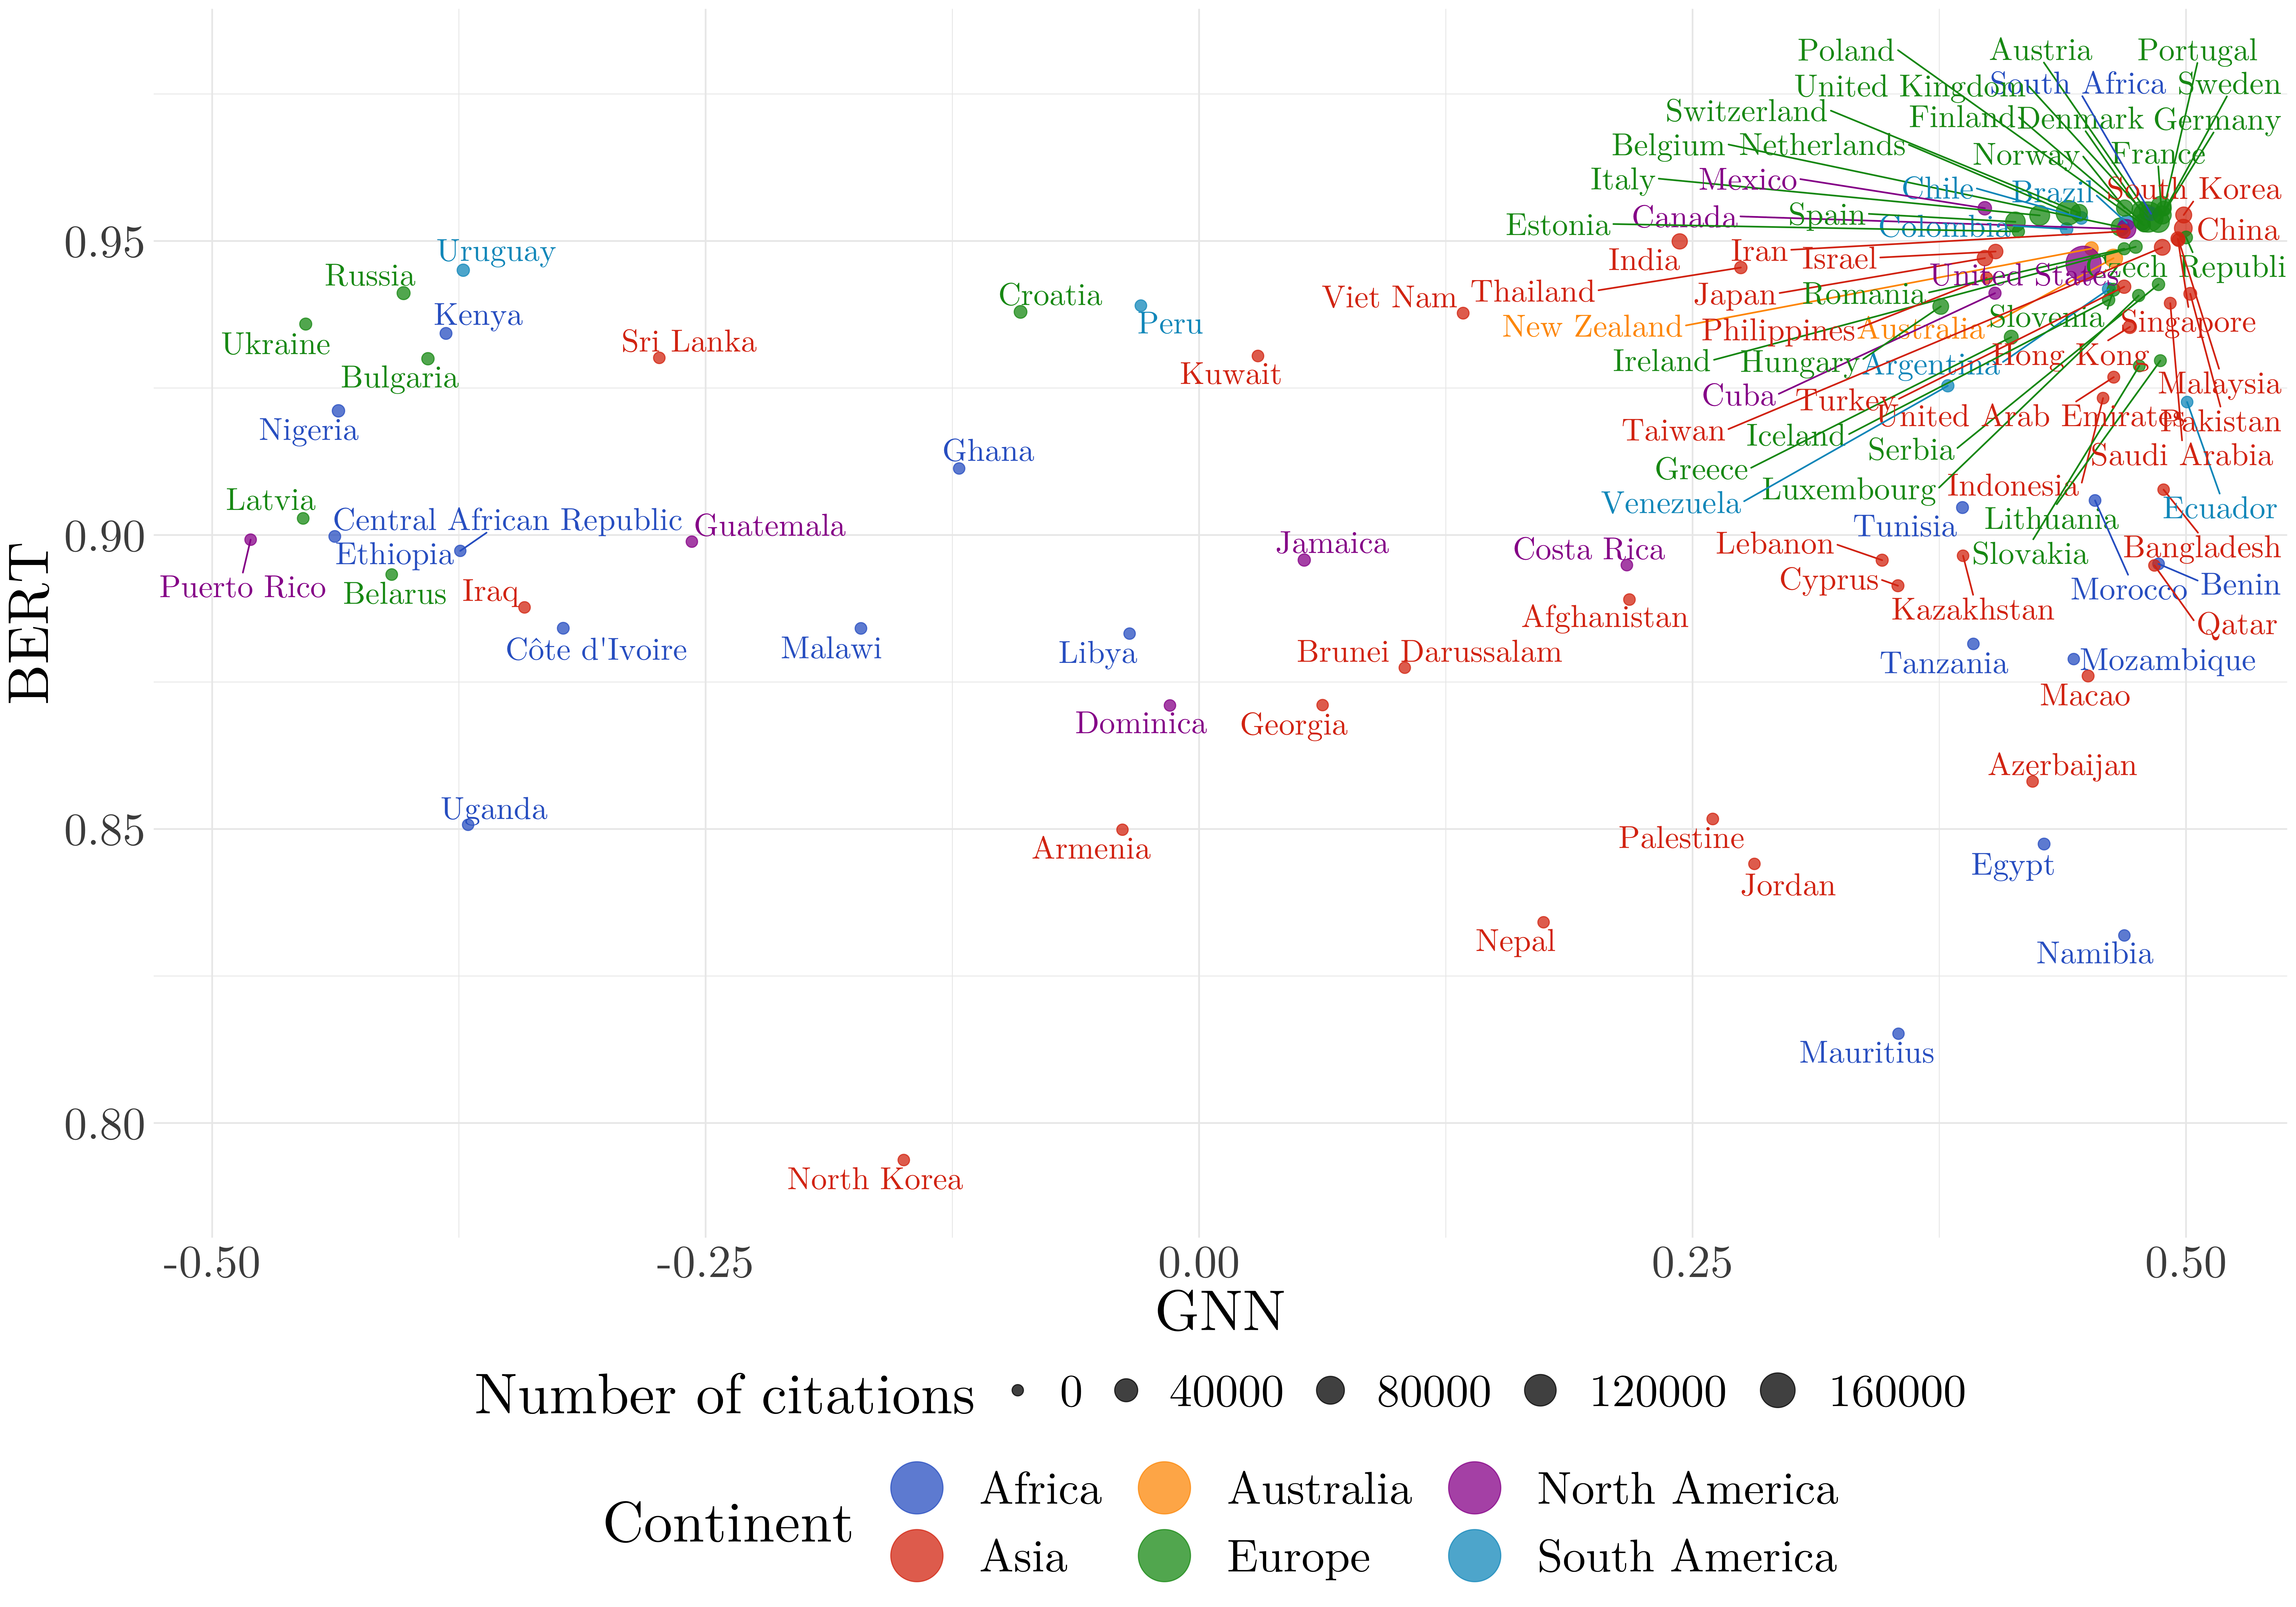
\includegraphics[width=\linewidth]{Fig6}
		\caption{Average cosine similarity by countries. BERT and GNN. Size by number of citations.}
		\label{fig:average_embedding}
	\end{figure}
	
	
	
	With the analysis of collaboration patterns, the Frobenius norm, and the country-level analysis, we can answer the research question {\sf RQ3}: How is the concept of \textit{prestige} expressed in the articles' embeddings?
    The idea of \textit{prestige} is strongly captured by the GNN embeddings. This concept unfolds into different expressions, such as the different position articles have in the embedding according to their collaboration patterns and citation levels, and also on hierarchical levels of analysis, like the distribution of countries.
	
	%------------------------------------------------------------------------------
	%------------------------------------------------------------------------------

	
	\pagebreak
	
	%TC:ignore 
	\printbibliography
	
	\pagebreak	
	\begin{appendices}
		
		%redifine tables and figures caption
		\renewcommand{\thetable}{\thesection\arabic{table}}
		\renewcommand\thefigure{\thesection.\arabic{figure}}    
		
		\section{Glossary} \label{sec:glossary}
		
		%restart table and fig counter after each appendix
		\setcounter{table}{0}
		\setcounter{figure}{0}    
		\begin{table}[!t]
			\centering
			\caption{Glossary of acronyms}
			\label{table:glossary} 

			\captionsetup{justification=centering}
			\begin{tabular}{@{}ll@{}}
				\toprule
				Meaning                                                & Acronym \\ \midrule
				Natural Language Processing                            & NLP     \\
				Document-Term Matrix                                   & DTM     \\
				Graph Neural Networks                                  & GNN     \\
				Term Frequency - Inverse Document Frequency            & TF-IDF  \\
				Latent Dirichlet Allocation                            & LDA     \\
				Recurrent Neural Network                               & RNN     \\
				Convolutional Neural Networks                          & CNN     \\
				Convolutional Graph Networks                           & CGN     \\
				Graph Convolutional Networks                           & GCN     \\
				Graph Isomorphic Network                               & GIN     \\
				Graph Attention Network                                & GAT     \\
				Attention-based Graph Neural Networks                  & AGNN    \\
				Graph Autoencoder                                      & GAE     \\
				Area Under the Receiver Operating Characteristic Curve & AUC     \\
				Average Precision                                      & AP      \\
				True Positive Rate                                     & TPR     \\
				False Positive Rate                                    & FPR     \\ \bottomrule
			\end{tabular}
		\end{table}
		
		\pagebreak
		
		
		\section{Data statistics. In and Out of Network}\label{sec:oon_stats}
		%restart table and fig counter after each appendix
		\setcounter{table}{0}
		\setcounter{figure}{0}    
		
		In this section, we split the table \ref{table:network_stats} between those articles that are part of the network in Table \ref{table:in_the_net}, and those that have no information about references and are not referenced by any other article, in Table \ref{table:out_of_net}. We can see that 75\% of articles are part of the network, and compared to those out of the network, they have a higher mean citation. Most of the articles that cannot be included in the network are from `Synthese' (30\%), `Research Policy'(12\%), or `Science and Public Policy' (11\%).
		
		
		% Please add the following required packages to your document preamble:
		% \usepackage{multirow}
		\begin{table}[!t]
			\centering
			\caption{Articles out of the network summary statistics.}
			\label{table:out_of_net}

			\resizebox{\textwidth}{!}{%
				\begin{tabular}{llrrr}
					\toprule
					Field & Journal & \begin{tabular}[c]{@{}r@{}}Articles\\ Retrived\end{tabular} & \begin{tabular}[c]{@{}r@{}}Mean\\ Citations\end{tabular} & \begin{tabular}[c]{@{}r@{}}Max\\ Citations\end{tabular} \\ \midrule
					\multirow{2}{*}{Management}                                                                             & Research Policy                                                                         & 643                                                         & 79.72                                                    & 3404                                                    \\
					& Science And Public Policy                                                               & 637                                                         & 10.31                                                    & 409                                                     \\ \hline
					\multirow{2}{*}{\begin{tabular}[c]{@{}l@{}}Library and \\ Information Sciences\end{tabular}}            & Scientometrics                                                                          & 784                                                         & 19.73                                                    & 435                                                     \\
					& Journal Of Informetrics & 12                                                          & 13.50                                                    & 28                                                      \\ \hline
					\multirow{8}{*}{History and Philosophy}  & Synthese                                                                                & 1702                                                        & 6.70                                                     & 564                                                     \\
					& \begin{tabular}[c]{@{}l@{}}Studies In History And \\ Philosophy Of Science\end{tabular} & 372                                                         & 7.68                                                     & 63                                                      \\
					& Isis & 250                                                         & 9.09                                                     & 123                                                     \\
					& Science And Education & 250                                                         & 10.92                                                    & 298                                                     \\
					& \begin{tabular}[c]{@{}l@{}}British Journal For\\ The History Of Science\end{tabular}    & 145                                                         & 9.03                                                     & 54                                                      \\
					& Social Studies Of Science & 139                                                         & 24.71                                                    & 648                                                     \\
					& Science, Technology And Society & 134                                                         & 4.15                                                     & 47                                                      \\
					& Science And Technology Studies   & 8                                                           & 2.25                                                     & 8                                                       \\ \hline
					\multirow{5}{*}{\begin{tabular}[c]{@{}l@{}}Education, \\ Communication and\\ Anthropology\end{tabular}} & Public Understanding Of Science                                                         & 170                                                         & 25.32                                                    & 416                                                     \\
					& Research Evaluation                                                                     & 142                                                         & 6.15                                                     & 76                                                      \\
					& \begin{tabular}[c]{@{}l@{}}Science, Technology\\ And Human Values\end{tabular}          & 106                                                         & 19.51                                                    & 272                                                     \\
					& Minerva & 79 & 7.24 & 78 \\ \hline
					& Total & 5573 & 16.00 & 3404 \\ \bottomrule 
				\end{tabular}
			}
		\end{table}
		
		\begin{table}[!t]
			\centering
			\caption{Articles in the network summary statistics.}
			\label{table:in_the_net}

			\resizebox{\textwidth}{!}{%
				\begin{tabular}{llrrr}
					\toprule
					Field & Journal & \begin{tabular}[c]{@{}r@{}}Articles\\ Retrived\end{tabular} & \begin{tabular}[c]{@{}r@{}}Mean\\ Citations\end{tabular} & \begin{tabular}[c]{@{}r@{}}Max\\ Citations\end{tabular} \\ \midrule
					\multirow{2}{*}{Management} & Research Policy & 2578 & 84.75 & 4820 \\
					& Science And Public Policy & 1070 & 15.03 & 462 \\ \hline
					\multirow{2}{*}{\begin{tabular}[c]{@{}l@{}}Library and\\ Information Sciences\end{tabular}} & Scientometrics & 4352 & 20.10 & 1334 \\
					& Journal Of Informetrics & 864 & 22.76 & 352 \\ \hline
					\multirow{8}{*}{History and Philosophy} & Synthese & 2449 & 9.80 & 910 \\
					& Social Studies Of Science & 930 & 43.38 & 4709 \\
					& Science And Education & 784 & 11.82 & 177 \\
					& \begin{tabular}[c]{@{}l@{}}Studies In History\\ And Philosophy Of Science\end{tabular} & 539 & 9.50 & 145 \\
					& Isis & 273 & 15.57 & 415 \\
					& Science, Technology And Society & 211 & 7.28 & 122 \\
					& \begin{tabular}[c]{@{}l@{}}British Journal\\ For The History Of Science\end{tabular} & 131 & 10.16 & 88 \\
					& Science And Technology Studies & 103 & 5.52 & 39 \\ \hline
					\multirow{5}{*}{\begin{tabular}[c]{@{}l@{}}Social Sciences:\\ Education, Communication\\ and Anthropology\end{tabular}} & Public Understanding Of Science & 807 & 26.04 & 518 \\
					& \begin{tabular}[c]{@{}l@{}}Science, Technology\\ And Human Values\end{tabular} & 651 & 35.04 & 828 \\
					& Research Evaluation & 524 & 15.04 & 223 \\
					& Minerva & 312 & 18.86 & 624 \\ \hline
					& Total & 16578 & 21.92 & 4820 \\ \bottomrule 
				\end{tabular}
			}
		\end{table}
		
		\pagebreak
		
		%------------------------------------------------------------------------------
		\section{Models definitions}
		%------------------------------------------------------------------------------
		%restart table and fig counter after each appendix
		\setcounter{table}{0}
		\setcounter{figure}{0}    
		
		%------------------------------------------------------------------------------
		\subsection{LDA}
		\label{sec:lda_def}
		%------------------------------------------------------------------------------
		As a generative Bayesian model, LDA states a generative process in which data is created, and then uses Bayes theorem to fit the parameters. The generative process is as follows:
		
		\begin{itemize}
			\item Each topic is generated as a multinomial distribution, $\beta_i$, over words
			\item For each document in the corpus, the words are defined in a two-step process:
			\begin{enumerate}
				\item First, we define the distribution of topics in the document as a multinomial distribution, $z$,
				\item for each word:
				\begin{itemize}
					\item randomly select a topic from the given $z$ distribution,
					\item given the topic, randomly select the word from the corresponding $\beta$ distribution.
				\end{itemize}
			\end{enumerate}
		\end{itemize}
		
		If we have a dictionary of $V$ possible words, $n$ documents, and $k$ topics. $\beta$ will be a matrix of $kxV$, where each row is the realisation of a Dirichlet process, i.e., a stochastic process where its realisations are multinomial distributions. $\beta$ will indicate the distribution of words over topics. $Z$ will be a matrix of $nxk$ which will indicate the distribution of topics over documents. $\beta$ and $Z$ are the desired outputs, but the corpus only gives us the actual words of documents. If we consider these documents as a realisation of this chained random processes, we can use the Bayes Theorem to infer the probabilistic distributions: 
		
		$$
		p(\theta,z|w,\alpha,\beta) = \frac{p(\theta,z,w|\alpha,\beta)}{p(w|\alpha,\beta)}
		$$
		
		where $\theta$ is the Dirichlet process that defines the distribution of topics over documents, $z$, and $\alpha$ is its parameter.
		
		%------------------------------------------------------------------------------
		\subsection{GNN Models}
		\label{sec:gnn_models}
		%------------------------------------------------------------------------------
		Figure \ref{fig:timeline} shows a synthesis of the different approaches taken to solve this issue. The first approaches were based on building sequences using random walks \cite{perozzi_deepwalk_2014}, or recurrent models \cite{scarselli_graph_2009}. After this, Graph Convolutions were defined using spectral methods \cite{bruna_spectral_2014} and spatial methods \cite{hamilton_inductive_2017}. More recently, new architectures were proposed that incorporate attention mechanisms \cite{velickovic_graph_2018}, U-nets \cite{gao_graph_2019} and autoencoders \cite{kipf_variational_2016}. For the remaining of this section, we present these models' intuitions, for an in-depth literature review, we refer the readers to \cite{hamilton_representation_2017,bacciu_gentle_2020, zhou_graph_2018,wu_comprehensive_2020}.
		
		\begin{figure}[!t]
			\centering
			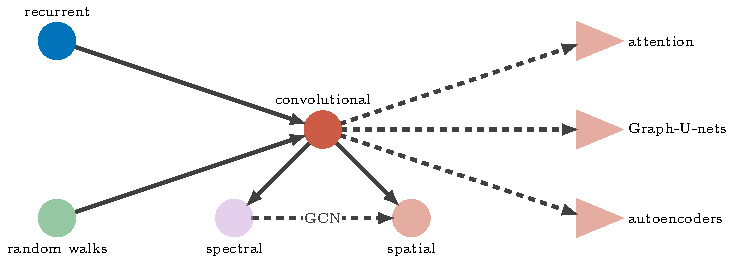
\includegraphics[width=.75\linewidth]{FigC1} 	
% 			\begin{tikzpicture}[scale=1.5]
% 			\Vertex[label=recurrent,x=0,position=90, style= {color = frenchblue}]{B}
% 			\Vertex[label=random walks,x=0,y=-2,position=-90, style= {color = etonblue}]{A}
% 			\Vertex[label=convolutional,x=3, y =-1,position=90, style={color = darkcoral}]{C}
% 			\Vertex[label=spectral,x=2, y=-2,position=below, style={color = wisteria,opacity =.5}]{D}
% 			\Vertex[label=spatial,x=4,y=-2,position=below, style={color = darkcoral,opacity =.5}]{E}
% 			\Vertex[label=autoencoders,x=6,y=-2,position=right,shape= isosceles triangle, style={color = darkcoral,opacity =.5}]{F}
% 			\Vertex[label=Graph-U-nets,x=6,y=-1,position=right,shape= isosceles triangle, style={color = darkcoral,opacity =.5}]{G}
% 			\Vertex[label=attention,x=6,y=0,position=right,shape= isosceles triangle, style={color = darkcoral,opacity =.5}]{H}
% 			%\Text[x=5, y=-1,width=1.5cm, color = darkcoral]{state of the art}
			
% 			\Edge[Direct](A)(C)
% 			\Edge[Direct](B)(C)
% 			\Edge[Direct](C)(D)
% 			\Edge[Direct](C)(E)
% 			\Edge[Direct, style = dashed](C)(H)
% 			\Edge[Direct,label=GCN, style = dashed](D)(E)
% 			\Edge[Direct, style = dashed](C)(F)
% 			%\Edge[Direct,label=GAE, style = dashed]()(F)
% 			\Edge[Direct,style = dashed](C)(G)
			
% 			\end{tikzpicture}
			\caption{Graph Neural Networks framework}
			\label{fig:timeline}
		\end{figure}
		
		\subsubsection{First Approaches}
		In this section, we briefly present the first approaches for GNN. These models are not used in the subsequent experiments, as they are not currently the state of the art. Nevertheless, they are all conceptually important.
		
		For the task of \textit{node embedding}, given the developments on Word Embeddings \cite{mikolov_linguistic_2013}, one of the first strategies proposed was to use random walks over nodes to define a sequence that can be later used as the input for a Word2Vec model, as it is normally done with texts on NLP. The first model that proposed this technique was DeepWalk \cite{perozzi_deepwalk_2014}. Later, \cite{grover_node2vec_2016} proposed node2vec, which defines flexible biased random walks, that includes parameters for adjusting the path taken by the random walks to search for structural roles or community structures. The major problem with these approaches is that they do not consider the features of the nodes, so they miss potentially useful information.
		
		\cite{scarselli_graph_2009} proposed the Graph Neural Network model which iteratively updates the nodes' state looking at its neighbours, until it converges. This recurrent model uses a single layer  which is iteratively updated. 
		
		Convolutional Graph Networks (CGN) models instead use a stack of layers. In this way, the number of updates is fixed, and the parameters of each layer are allowed to change, giving more flexibility to the model. 
		Spectral-based methods were the first type of CGN \cite{bruna_spectral_2014}. They use the \textit{graph Fourier transform} on the Laplacian matrix (a normalised adjacency matrix), which can be thought of as the effect of a signal over the network. This model, while conceptually important, suffers from many problems. In particular, as it uses the full graph structure, it can only work on transductive settings, i.e., it cannot be used on a different graph on train and test. More importantly, the eigen-decomposition requires $\mathcal{O}(n^3)$ where $n$ is the number of nodes. This is prohibitively expensive when the network has billions of nodes, like social networks.
		
		\subsubsection{State Of The Art}
		In this section, we present the current state of the art in GNN.  A combination of these models will be used in the experimental analysis for the task of link prediction. 
		
		\paragraph{GCN}
		
		Many models improve the limitations present in the spectral method proposed by \cite{bruna_spectral_2014}. \cite{defferrard_convolutional_2016} build an approximation of the original model with Chebyshev polynomials. \cite{kipf_semi-supervised_2017} introduce the \textit{Graph Convolutional Networks} (GCN), which further reduces the model and includes self-connections, this means that in the iterative process of building a representation based on its neighbours, the node will also look at itself, which is a desirable property.  The GCN simplifies the model by only looking at the first-order neighbourhood. If the representation of a node is initiated with its feature vector, the GCN update builds an average representation based on itself, due to self-connections, and its neighbours. Instead of iterating the update step until convergence, like recurrent models, in GCN a stack of layers is built. The stacking of GCN layers allows the  node representation to be based on more distant nodes. Here, simplicity is the key for building a powerful model. 
		
		\paragraph{GraphSage}
		
		\cite{hamilton_inductive_2017} propose several variations over the GCN, in the  \textit{GraphSage} model. As the formulation of the problem can be useful for understanding how Graph Convolutional Networks works, we present their algorithm in \ref{alg:graphsage} . The model needs the following inputs:
		
		\begin{itemize}
			\item The Graph $\mathcal{G}(\mathcal{V},\mathcal{E})$ with a list of vertices $\mathcal{V}$ and edges $\mathcal{E}$, and
			\item the input features $x$, where $x_v$ is the feature vector of the node $v$.
		\end{itemize}
		
		We also need to define the number of layers the model will have, $K$, a set of weight matrices $W^k$ for each layer (that will be later trained with the data), and an activation function $\sigma$. We also need a way in which a group node embeddings will be aggregate, and a way of defining the neighbourhood of a node.  
		
		The model starts the node embeddings with their feature vectors. After this, in each of the $K$ layers, for each node $v \in \mathcal{V}$, it first defines its neighbours. One of the changes with respect to GCN is that GraphSage samples a fixed amount of neighbours to control the computational footprint. Given the neighbourhood, the $AGGREGATE$ function is used to build a new vectorised representation of those (line 4), and this is later concatenated with the embedding of node $v$ in the previous layer (line 5). A projection is made with the $W^k$ matrix, and also an activation layer is used. This correspond with the typical structure of a deep learning layer. When the model is fitted with back-propagation for a specific task, the $W^k$ are updated in order to optimise the lost function \cite{kelley_gradient_1960}. Line 6 is simply a regularisation.
		
		\begin{algorithm}[!t]
			\caption{GraphSAGE \cite{hamilton_inductive_2017}}
			\label{alg:graphsage}
			\hspace*{\algorithmicindent{  \textbf{Input:} Graph $\mathcal{G}(\mathcal{V},\mathcal{E})$: input features $x$ ; depth K ; weight matrices $W^k, \forall k \in {1,...,K}$; nonlinearity $\sigma$ ; differentiable aggregator functions $AGGREGATE_k, \forall k \in {1,...,K}$; neighbourhood function $\mathcal{N}: v \to 2^\mathcal{V}$.}}\\
			\hspace*{\algorithmicindent}  \textbf{output}  Vector representations $z_v \forall v \in \mathcal{V}$.
			\begin{algorithmic}[1]
				
				\State $h_v^0 \leftarrow x_v, \forall v \in \mathcal{V}$;
				\For {$k= 1\dots K$}
				\For {$v \in \mathcal{V}$}
				\State $h_{\mathcal{N}(v)}^k \leftarrow AGGREGATE_k(\{h_u^{k-1},\forall u \in \mathcal{N}(v)\})$;
				\State $h_v^k \leftarrow \sigma(W^k CONCAT(h_v^{k-1}, h_{\mathcal{N}(v)}^k))$
				\EndFor
				\State  $h_v^k \leftarrow h_v^k/||h_v^k||_2, \forall v \in \mathcal{V}$
				\EndFor
				\State $z_v \leftarrow h_v^K, \forall v \in \mathcal{V}$		
			\end{algorithmic}
		\end{algorithm}
		
		Depending on the election of the AGGREGATE and the CONCAT operators, this model is an approximation of GCN from \cite{kipf_semi-supervised_2017}. If we use the \textit{mean} as an aggregation function, and instead of concatenating $h_v^{k-1}$ and $h_{\mathcal{N}(v)}^k$ we average them, this is exactly the GCN model. The authors also propose two other aggregators: the \textit{LSTM aggregator} which can be more expressive, although the LSTM model (a RNN) requires a sequential order in the inputs, so the authors need to define an ad hoc order for the neighbours. And the \textit{pooling aggregator} in which the neighbours vector representation is fed through a fully connected layer and then the max-pooling is applied.
		
		\paragraph{GIN}
		Recent studies analyse the relation between GNN and the Weisfeiler-Lehman test of isomorphism \parencite{xu_how_2019}. Two graphs are isomorphic if they are topologically identical. Besides the embedding representation of nodes, it is also possible to build embedding representations of the entire graph. In the previous framework, we would need to add a READOUT operation that takes the nodes embedding as input and generates a single embedding representation for the entire network. If for two graphs $G_1$ and $G_2$ that are non-isomorphic we can build a different embedding representation, we are able to distinguish between those two. \cite{xu_how_2019} proves that the GNN power for discriminating between non-isomorphic networks is at most that of the Weisfeiler-Lehman test. However not every GNN can have this power, the \textit{Graph Isomorphic Network} (GIN) is a proposal that achieves the maximum discriminative capacity by using a specific update function, which replaces the $AGGREGATE$ functions proposed by \cite{hamilton_inductive_2017} (\textit{mean}, \textit{LSTM} or \textit{max}) with a \textit{summation} over the neighbourhood. This model has the advantage of a theoretically robust decision on the AGGREGATE function. 
		
		\paragraph{GAT}
		In GCN, nodes embeddings are updated using their neighbours embedding. Up to this point, all models consider that every neighbour has the same influence, which might not be true. \textit{Graph Attention Networks } (GAT) \cite{velickovic_graph_2018} use attention mechanisms (which are currently state of the art in other problems, like NLP) to assign a different influence to each neighbour. The update of the node representation becomes:
		
		$$
		h_v = \sigma (\sum_{u \in \mathcal{N}(v)} \alpha_{u,v}Wh_u)
		$$
		
		where $W$ is still a learning weight matrix and $\alpha_{u,v}$ is the normalised attention between nodes $u$ and $v$.
		
		Following \cite{vaswani_attention_2017}, GAT uses \textit{multihead attention}, which implies applying $K$ independent attentions and concatenating their results (except for the final layer, where they are averaged).
		
		This model has the advantage of learning the different importance of the neighbours, given their feature vector. Moreover, the attention mechanisms have the potential of an increasing interpretabilty of the mode. \cite{thekumparampil_attention-based_2018} propose a variation of this model, \textit{Attention-based Graph Neural Networks} (AGNN), where the \textit{relevance} is defined based on the cosine similarity.
		
		\paragraph{GraphUNet} \cite{gao_graph_2019} proposed GraphUNet, based on a new definition of Pooling layers. Convolutional layers in computer vision are normally used with \textit{Pooling layers}. This is because the convolutional filters are trained to detect the presence of a specific feature in a portion of the image, and if the feature is found, the result will have high positive values. The max pooling layer, makes a downsizing of the input and captures the highest values. By doing this, it generates a clear indication whether or not that particular feature was present.
		However, as it happens with traditional convolutions, the pooling layers are defined based on the regular pattern of the image. Defining a pooling layer on the graph domain could be useful for building better representations of hierarchical patterns.
		\cite{gao_graph_2019} proposed a new definition of pooling \textit{gPool}. The gPool layer makes a linear projection of the nodes features, and a $k$-max pooling selection. With the identifier of the selected nodes, it builds the new (reduced) adjacency matrix and feature matrix. \cite{gao_graph_2019} also proposes an unpooling layer, which rebuilds the original network, and used together they can build an encoder-decoder architecture. The benefit of such an architecture is that it lets the node embedding be built based on the hierarchical properties of their neighbourhood. 
		
		\paragraph{Autoencoders}
		
		The Autoencoder is an architecture in deep learning where the network tries to learn the input, but goes through a compressed state. The network can be divided into two elements:
		
		\begin{itemize}
			\item the encoder, which can be a regular stack of layers, that ends with a vectorised representation of the input,
			\item the decoder, where the representation received from the encoder will be sized up to the original form. 
		\end{itemize}
		
		The idea is that, if the network is able to reconstruct the original input with a small error margin, then most of the information from the original input is correctly compressed in the low dimension at the end of the encoder.
		
		\cite{kipf_variational_2016} proposed the Graph Autoencoder (GAE) and the Variational GAE (a probabilistic implementation of the GAE), where the encoder can be any way of building a node embedding, like a stack of GCN layers, and the decoder is (for the GAE) the reconstructed adjacency matrix, $\hat{A}$:
		
		\begin{equation*}\label{GAE}
		\hat{A} = \sigma(ZZ^T), \qquad \text{with} \quad Z = GCN(X,A)
		\end{equation*}
		
		Where $Z$ represents the embedding matrix built using the GCN and $\sigma$ is a logistic sigmoid function. The model use the inner product of the node embeddings to reconstruct a probabilistic adjacency matrix. This transforms the embedding into edge probabilities for the given node pairs. This is a particularly useful architecture for the task of \textit{link prediction}.
		
		In this paper, we train our models for this task in a transductive setting. We randomly remove some citation links for test and validation set, and evaluate how well the reconstructed adjacency matrix can predict those removed links. We use as encoders the GCN, GraphSAGE, GIN, GAT, AGNN, and GraphUNet layers defined above, which constitute the current state of the art in the field.
		
		\section{Frobenius Norm}\label{sec:frobenius_norm}
		%restart table and fig counter after each appendix
		\setcounter{table}{0}
		\setcounter{figure}{0}    
		
		In Figure \ref{fig:frobeniousnorm}, we can see the Frobenius norm of the article's embedding by their citation level. For the GNN embedding we can see the higher norm of highly cited articles, while in the BERT embedding this does not sustain \footnote{Doc2Vec and LDA embeddings do not show significant differences between articles norms.}.
		
		\begin{figure}[htbp]
			\centering
			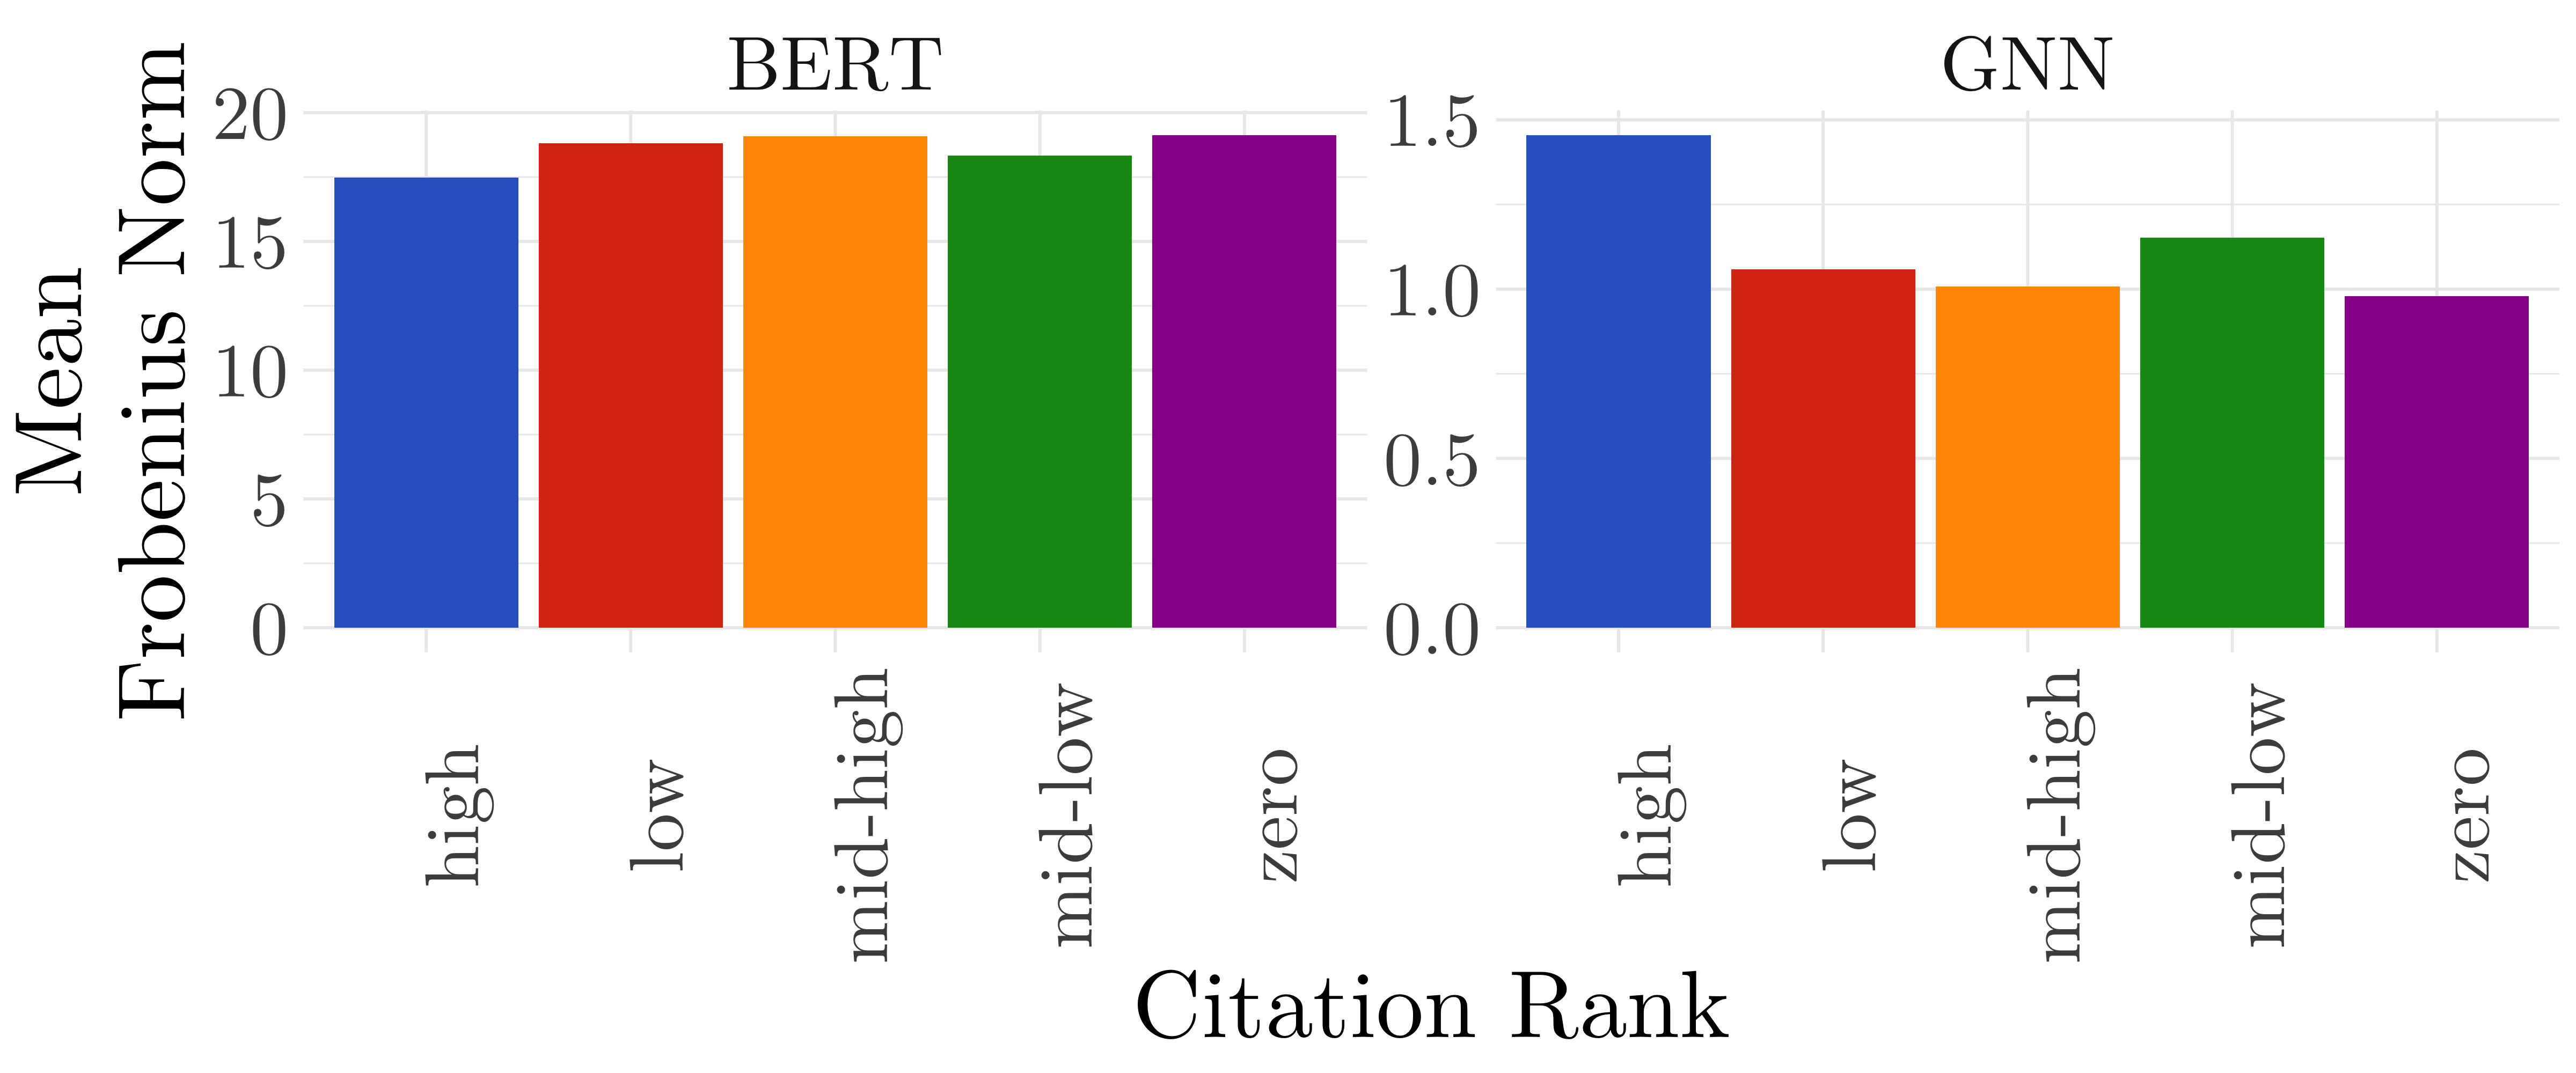
\includegraphics[width=\linewidth]{FigD1}
			\caption{Frobenius Norm of articles by citation level.}
			\label{fig:frobeniousnorm}
		\end{figure}
		
		
	\end{appendices}
	%TC:endignore 
	
\end{document}
